% !TeX root = ../thuthesis-example.tex

\chapter{系统架构设计与高性能实现}

本章从软件工程和系统优化的角度,详细阐述ReGen系统的架构设计原理和关键技术实现。针对4D高斯溅射与视频扩散模型融合的复杂性,本文提出了分层解耦的架构方案,并针对GPU内存限制、计算效率、数值稳定性等关键技术挑战,设计了一系列创新的工程解决方案。

\section{分层架构与渲染引擎}

本节阐述系统的整体架构设计思想和高性能渲染引擎的实现方案。从软件架构的角度分析4D场景重建系统的复杂性,本文提出了五层解耦架构来降低系统复杂度并提高可维护性,同时针对实时渲染的需求设计了多模态渲染管线和GPU加速优化策略。

\subsection{五层解耦架构设计}

针对4D高斯溅射与视频扩散模型融合的复杂性,本文提出了一种五层解耦架构,每层承担明确的职责并通过标准化接口进行交互。这种分层设计使得系统能够将复杂的技术挑战分解为可管理的模块,降低了系统复杂度,提高了可维护性,并支持组件级别的独立优化和测试,便于不同算法模块的替换和扩展。

数据抽象层负责输入数据的统一格式化和预处理,采用适配器模式屏蔽不同数据格式的差异。几何表示层负责4D高斯溅射的核心数据结构管理,采用组合模式统一处理静态背景、动态物体和环境表示,为上层提供一致的几何查询接口。神经渲染层实现了可微分高斯光栅化引擎,采用策略模式支持多种渲染后端,既可以使用CUDA加速的高性能渲染器,也可以切换到Python实现的调试版本。扩散推理层封装了视频扩散模型的推理逻辑,实现了内存高效的长序列采样算法,通过滑动窗口机制和键值缓存技术支持任意长度视频的生成。扩散监督层协调扩散模型和4DGS的联合优化,实现了自适应的监督信号传递算法,根据训练状态动态调整扩散采样的频率和强度。

\begin{figure}[htbp]
  \centering
  \includegraphics[width=0.95\textwidth]{pdf/system_architecture.pdf}
  \caption{ReGen系统五层架构设计}
  \label{fig:system-architecture}
\end{figure}

为了确保各层之间的松耦合,系统设计了标准化的接口协议。数据传输接口定义了Camera、PointCloud、Trajectory等核心数据结构,确保数据在不同模块间的一致性传递,所有空间坐标统一采用右手坐标系,时间戳统一为纳秒精度。渲染接口抽象了渲染操作的核心接口,支持不同渲染后端的透明切换,通过统一的RenderConfig类管理渲染参数,使得上层算法无需关心底层实现细节。优化接口定义了统一的参数更新和梯度传播接口,支持不同优化器和学习率调度策略的灵活配置,通过标准的backward()和step()接口实现与PyTorch生态的无缝集成。

\subsection{多模态渲染管线设计}

系统设计了一种多模态渲染管线,能够同时处理静态背景、动态物体和环境映射三种不同类型的几何表示。该设计的核心创新在于组件化渲染策略,将复杂的场景渲染分解为多个独立的渲染通道,每个通道专注于特定类型的几何表示,最后通过可配置的组合函数生成最终渲染结果。

数学上,将渲染过程建模为一个可配置的组合函数:

\begin{equation}
\mathcal{R}_{\text{total}}(\pi, \mathcal{G}) = \mathcal{C}(\mathcal{R}_{\text{bkgd}}(\pi, \mathcal{G}_{\text{bkgd}}), \mathcal{R}_{\text{obj}}(\pi, \mathcal{G}_{\text{obj}}), \mathcal{R}_{\text{sky}}(\pi, \mathcal{G}_{\text{sky}}))
\label{eq:modular_rendering}
\end{equation}

其中$\mathcal{C}$是可配置的组合函数,支持不同的混合策略和后处理操作。静态背景渲染器$\mathcal{R}_{\text{bkgd}}$负责处理不随时间变化的场景元素,如建筑物、道路和植被,通过跨时间帧的几何聚合来提高表示密度。动态物体渲染器$\mathcal{R}_{\text{obj}}$处理运动的车辆和行人,每个物体维护独立的高斯基元集合,并通过刚体变换描述其运动轨迹。天空渲染器$\mathcal{R}_{\text{sky}}$采用专门的环境映射技术,通过球谐函数或立方体贴图表示天空的光照和颜色分布。

\begin{figure}[htbp]
  \centering
  \includegraphics[width=0.95\textwidth]{pdf/rendering_modes.pdf}
  \caption{多模态渲染架构与渲染模式}
  \label{fig:rendering-modes}
\end{figure}

\subsection{GPU加速的光栅化优化}

针对4D高斯溅射的计算特点,系统设计了多项GPU加速优化策略以实现实时渲染性能。基于tile的渲染策略将图像分割为$16 \times 16$的tile,每个tile独立处理,充分利用GPU的并行计算能力,使得渲染过程可以在多个CUDA线程块中同时进行。自适应排序优化设计了基于深度和不透明度的自适应排序算法,通过提前终止策略减少不必要的计算开销,当累积不透明度接近1时即停止该像素的进一步计算。内存池管理实现了GPU内存池管理机制,预分配内存块并重复使用,避免了频繁的内存分配和释放操作带来的性能开销。

内存池的大小根据场景复杂度动态调整,通过经验公式估算所需内存:

\begin{equation}
M_{\text{pool}} = \alpha \cdot N_g \cdot D_{\text{gaussian}} + \beta \cdot H \cdot W \cdot C + M_{\text{buffer}}
\label{eq:memory_pool_sizing}
\end{equation}

其中$\alpha$和$\beta$是经验系数,分别设置为1.2和1.1以提供适当的内存余量,$N_g$是高斯基元数量,$D_{\text{gaussian}}$是单个高斯基元的参数大小,$H \times W$是渲染分辨率,$C$是颜色通道数,$M_{\text{buffer}}$是安全缓冲区大小。这种动态内存管理策略使得系统能够在保证渲染质量的前提下,有效利用有限的GPU内存资源。

\section{扩散模型的系统集成与优化}

本节详细阐述扩散模型在系统中的集成方式和针对长序列视频生成的优化策略。系统采用了基于Wan2.2-I2V-A14B的Diffusion Transformer架构,通过自适应采样调度和训练自由引导机制实现了高效的扩散监督训练,同时针对长视频序列处理的内存挑战设计了滑动窗口机制和键值缓存策略。

\subsection{自适应采样调度与训练自由引导}

本文提出了一种自适应的扩散采样调度算法,根据4DGS模型的训练状态动态调整采样频率和引导强度。该算法的核心思想是在训练早期提供强引导以建立正确的几何结构,在训练后期减弱引导以保持模型的自主学习能力。动态采样频率调整采用高斯衰减的策略,在训练的关键阶段增加采样频率,在稳定阶段减少采样以提高训练效率。这种调整策略基于训练损失的变化趋势和模型收敛状态,能够自动识别需要重点优化的训练阶段。

引导强度的衰减采用渐进式策略,从初始的强引导逐渐减弱到后期的弱引导,随着训练的进行逐步降低扩散模型的引导权重。这种设计确保了模型在训练初期能够快速学习到正确的几何结构,同时在训练后期保持足够的自主学习能力,避免过度依赖外部引导而影响模型的泛化性能。

训练自由引导机制是一种自适应的正则化策略,通过引入当前模型状态作为额外的先验信息,防止扩散监督训练过程中的模式崩溃。该机制的核心优势在于能够动态调整引导信号的强度,根据当前模型的渲染质量来决定扩散模型引导的权重。系统会实时评估当前4DGS模型的渲染质量,当质量较低时增强扩散引导,当质量较高时减弱引导强度。这种自适应调整策略确保了训练过程的稳定性,同时避免了过度引导可能导致的模型退化问题。

\subsection{Diffusion Transformer架构适配}

系统采用了基于Wan2.2-I2V-A14B的Diffusion Transformer架构,该架构相比传统的U-Net设计在视频生成任务中具有显著优势。DiT架构将视频的潜在表示分割为补丁序列,通过自注意力机制捕捉时空长程依赖关系。在补丁化处理方面,视频潜在表示被分割为固定大小的时空补丁,这种分割策略使得DiT能够将复杂的视频数据转换为序列形式,充分利用Transformer架构在序列建模方面的优势。补丁大小的选择需要在计算效率和表示精度之间找到平衡,在时间维度上保持较小的分割粒度以捕捉细粒度的运动模式,在空间维度上使用较大的分割以控制序列长度。

系统集成了Wan2.2的混合专家(MoE)架构创新,采用基于信噪比的专家路由策略。高噪声专家负责处理扩散过程的早期阶段,专注于整体布局和动态构建,学习场景的全局结构和粗粒度运动模式。低噪声专家处理后期精细化阶段,专注于细节优化,学习纹理、光照等精细视觉特征。这种分工策略使得模型能够在不同的去噪阶段采用最适合的处理方式,提升了整体的生成质量和效率。MoE机制通过增加模型容量而不显著增加计算成本,使得系统能够在保持推理效率的同时获得更强的表达能力。

\subsection{内存高效的长序列处理}

DiT架构在处理长视频序列时面临自注意力计算的二次复杂度挑战。为了解决这一问题,系统采用滑动窗口机制将长视频序列分割为重叠的时空窗口,在每个窗口内进行完整的自注意力计算。这种方法既保持了DiT架构捕捉长程依赖的优势,又有效控制了内存占用。系统设计的滑动窗口策略考虑了视频数据的时空特性。在时间维度上,窗口大小根据可用GPU内存和序列长度动态调整,确保每个窗口都能在内存限制内完成计算。在空间维度上,我们保持DiT原有的补丁分割方式,将每帧图像分割为固定大小的补丁序列。

为了保证相邻窗口间的时间连续性,系统采用适当的重叠策略,即相邻窗口之间共享部分时间帧。这种重叠设计确保了视频帧间的平滑过渡,避免了窗口边界处的不连续性问题。同时,我们通过键值缓存机制实现跨窗口的信息传递,使得模型能够利用历史窗口的计算结果。具体而言,当前窗口的注意力计算可以复用前一窗口重叠部分的键值对,避免重复计算,从而进一步提升了推理效率。

针对现代GPU架构,系统集成了内存高效的注意力计算。系统采用了优化的attention实现,并通过批处理优化来处理大规模序列。批处理大小根据当前GPU内存占用动态调整,在保证计算精度的前提下最大化内存利用率。通过这些优化策略的组合,系统能够在保持DiT架构优势的同时,有效处理长视频序列的生成任务。

\section{内存管理与并行计算架构}

本节阐述系统的内存优化策略和并行计算架构设计。针对4DGS和视频扩散模型的巨大内存需求,系统设计了分层内存管理策略和异步计算流水线。同时,为了确保训练过程的数值稳定性和收敛性,系统实现了多尺度数值稳定性保证机制和动态损失权重平衡策略。此外,针对4DGS的动态几何表示需求,本文提出了多准则密化决策算法。

\subsection{分层内存管理与并行计算}

针对4DGS和视频扩散模型的巨大内存需求,系统设计了分层内存管理策略。该策略通过对不同类型的数据采用差异化的内存管理方法,实现了系统内存使用的整体优化。参数内存优化采用混合精度存储策略,对计算敏感的参数(如高斯位置、协方差矩阵)保持FP32高精度,对其他参数(如颜色、不透明度)使用FP16较低精度以节省内存。中间激活管理实现了智能的激活值缓存策略,根据计算图的特点选择性地保存和释放中间结果,通过静态分析确定哪些中间激活在反向传播中需要使用,只保留这些必要的激活值。梯度检查点优化针对深度神经网络的反向传播特点,在内存占用和重计算成本之间找到最优平衡点,通过在网络的关键层设置检查点,在反向传播时重新计算中间激活,将内存占用从$O(L)$降低到$O(\sqrt{L})$,其中$L$是网络层数。

系统设计了异步计算流水线,将扩散采样、4DGS渲染、梯度计算等操作进行流水线化处理。这种设计的核心优势在于能够充分利用GPU的并行计算能力,通过重叠不同类型的计算操作来提升整体的训练效率。异步流水线的实现需要仔细协调不同计算任务的时序关系,确保数据依赖关系得到正确处理。我们使用CUDA流(Stream)机制实现不同操作的并发执行,扩散采样在Stream0上执行,4DGS渲染在Stream1上执行,两者可以并行进行。通过优化任务调度和内存访问模式,能够显著减少同步等待时间,使得总体训练时间接近最耗时操作的时间,而不是所有操作时间的累加。

\subsection{数值稳定性与收敛性保证}

4D高斯溅射涉及多个数量级的数值计算,从微米级的尺度参数到千米级的位置坐标,系统设计了多尺度数值稳定性保证机制。该机制的核心目标是确保训练过程中各种数值操作的稳定性,避免梯度爆炸、参数溢出等常见的数值问题。自适应梯度裁剪机制根据梯度的历史统计信息动态调整裁剪阈值,通过计算梯度范数的移动平均值和标准差,将裁剪阈值设置为$\bar{g} + 2\sigma_g$,其中$\bar{g}$是梯度范数的移动平均,$\sigma_g$是标准差。这种自适应策略既能防止梯度爆炸,又不会过度抑制有效的梯度信号。

参数约束机制确保高斯基元的各项参数始终保持在合理的数值范围内。位置参数$\boldsymbol{\mu}$被约束在场景边界内,通过软约束的方式施加边界损失,避免高斯基元漂移到场景之外。尺度参数$\mathbf{s}$被限制在$[s_{\min}, s_{\max}]$范围内,其中$s_{\min} = 0.0001$米防止高斯退化为点,$s_{\max} = 100$米防止过度膨胀。不透明度参数$\alpha$通过sigmoid函数自然约束在$(0, 1)$区间内。旋转四元数$\mathbf{q}$在每次更新后进行归一化,确保其保持单位范数。

为了确保训练过程的稳定收敛,系统实现了动态损失权重平衡机制。该机制能够自动调整不同损失项的相对权重,确保各个优化目标能够协调发展。权重调整策略基于各个损失项梯度幅度的相对关系,通过计算每个损失项对参数梯度的贡献度$g_i = \|\nabla_\theta \mathcal{L}_i\|_2$,将权重设置为$\lambda_i = \lambda_i^0 \cdot \bar{g} / g_i$,其中$\lambda_i^0$是初始权重,$\bar{g}$是所有损失项梯度的平均值。这种自适应调整机制确保了训练过程的平衡性和稳定性,避免某个损失项过度主导训练过程。

\subsection{自适应密化算法}

本文提出了一种多准则密化决策算法,综合考虑梯度统计、几何特征和时间一致性来指导高斯基元的动态调整。该算法的核心思想是通过多个维度的信息融合,实现更加智能和稳定的密化决策。在梯度统计方面,我们对高斯基元的位置梯度进行时间聚合,只考虑在当前时间窗口内可见的基元,避免被遮挡基元对统计结果的干扰。具体地,对于每个高斯基元$g_i$,我们计算其在最近$K$次迭代中的平均梯度$\bar{\nabla}_i = \frac{1}{K}\sum_{k=1}^K \nabla \boldsymbol{\mu}_i^{(k)}$,只有当$\|\bar{\nabla}_i\| > \tau_{\text{grad}}$时才考虑密化该基元。

几何特征分析包括各向异性度量、局部密度估计和可见性统计三个方面。各向异性度量反映了高斯基元形状的不规则程度,定义为$a_i = \max(\mathbf{s}_i) / \min(\mathbf{s}_i)$,当$a_i > \tau_{\text{aniso}}$时表示基元过度拉伸,需要进行分割操作。局部密度估计通过计算邻近基元的分布情况,识别需要增加细节的稀疏区域,对于每个基元计算其$k$近邻的平均距离$d_i = \frac{1}{k}\sum_{j \in \mathcal{N}_k(i)} \|\boldsymbol{\mu}_i - \boldsymbol{\mu}_j\|$,当$d_i > \tau_{\text{density}}$时表示该区域密度不足。可见性统计记录了基元在不同时刻的可见频率$v_i = \frac{1}{T}\sum_{t=1}^T \mathbb{I}[\text{visible}(g_i, t)]$,为剪枝操作提供依据,当$v_i < \tau_{\text{vis}}$时该基元可能是冗余的。

最终的密化决策通过加权融合这些多维度特征来实现。对于密化操作,当$w_1 \|\bar{\nabla}_i\| + w_2 a_i + w_3 d_i > \tau_{\text{densify}}$时执行密化,其中权重参数$\{w_1, w_2, w_3\}$根据训练阶段和场景特性进行动态调整。在训练早期增大$w_1$以更多依赖梯度信息,在训练后期增大$w_2$和$w_3$以更多考虑几何质量。这种自适应权重策略确保算法能够适应不同的训练条件和数据特点。

\section{分布式训练与推理部署}

本节详细阐述系统的分布式训练架构和推理部署方案。针对DiT模型的大规模参数和长序列特性,系统设计了融合FSDP和序列并行的分布式训练架构。同时,为了支持不同的部署场景,系统实现了灵活的多模式推理引擎,能够在单GPU和多GPU环境中进行自适应部署。

\subsection{分布式训练架构}

针对DiT模型的大规模参数和长序列特性,系统设计了融合FSDP(Fully Sharded Data Parallel)和序列并行的分布式训练架构。该架构充分考虑了Wan2.2-I2V-A14B模型的MoE特性和注意力计算的并行化需求。我们的分布式策略采用FSDP对DiT模型和T5文本编码器进行独立的参数分片管理,每个GPU只保存模型参数的一个分片,在前向传播时通过all-gather操作收集完整参数,在反向传播时通过reduce-scatter操作聚合梯度。这种参数分片策略将单GPU的内存占用从$O(M)$降低到$O(M/N)$,其中$M$是模型参数量,$N$是GPU数量,使得大规模模型的训练成为可能。

对于长序列注意力计算,系统采用Ulysses策略在序列维度进行并行化处理。Ulysses将序列维度分片到不同的GPU上,每个GPU处理序列的一个子集,通过all-to-all通信实现完整的注意力计算。这一策略要求注意力头数能被GPU数量整除,当这一约束条件不满足时,系统会自动切换至Ring策略,改为要求序列长度能被GPU数量整除。Ring策略通过环形通信模式逐步传递键值对,每个GPU依次计算与其他GPU分片的注意力,虽然通信次数增加但对硬件约束更加灵活。

针对MoE架构中可能出现的专家负载不均衡问题,系统实现了动态负载均衡机制。该机制通过监控各个专家的使用频率,动态调整路由策略,确保计算负载在不同GPU间的合理分配。具体而言,在路由概率中引入负载均衡项$\mathcal{L}_{\text{balance}} = \alpha \sum_{e=1}^E (\frac{n_e}{N} - \frac{1}{E})^2$,其中$n_e$是分配给专家$e$的样本数,$N$是总样本数,$E$是专家数量。这个损失项鼓励样本均匀分配到各个专家,避免某些专家过载而其他专家空闲。

\subsection{内存优化与容错机制}

系统集成了DeepSpeed ZeRO优化器,实现了参数、梯度和优化器状态的三级分片。ZeRO-1仅分片优化器状态,ZeRO-2额外分片梯度,ZeRO-3进一步分片模型参数。根据模型规模和GPU数量,我们动态选择合适的ZeRO等级,对于大规模Wan2.2模型,在多GPU环境中使用ZeRO-2即可满足内存需求,而在较少GPU数量下则需要使用ZeRO-3。这种分片策略能够显著降低单个GPU的内存占用,使得大规模模型的训练成为可能。同时,系统采用FP16混合精度训练配合动态损失缩放,在保持数值稳定性的前提下进一步优化内存使用,前向传播和大部分计算使用FP16,关键的归约操作和参数更新使用FP32以保证精度。

为了减少通信开销,系统实现了带有错误反馈机制的梯度压缩技术。该压缩方法能够在保持收敛性的同时,显著减少分布式训练中的网络通信量。系统采用Top-K稀疏化策略,只传输梯度中绝对值最大的$k$个元素,其余元素累积到误差缓冲区中,在后续迭代中补偿。这种方法在理论上可以保证与无压缩训练相同的收敛性,实验表明适当的稀疏率可以大幅减少通信量而几乎不影响收敛速度,特别是在带宽受限的环境中表现出明显的优势。

针对DiT模型的大参数量特性,系统设计了分层检查点策略。该策略将模型参数、优化器状态和随机种子分别管理,根据不同组件的重要性和变化频率设置不同的保存间隔。模型参数定期保存,优化器状态以较高频率保存(因为可以从模型参数重新初始化),随机种子每次改变时立即保存。这种分层设计在保证系统可靠性的同时,有效减少了检查点操作的开销。检查点间隔的选择需要在系统可靠性和计算效率之间找到平衡。我们通过分析历史故障数据和重计算成本,将检查点间隔设置为适当值,确保在系统故障时能够以最小的代价恢复训练状态。

\subsection{多模式推理引擎}

针对Wan2.2-I2V-A14B模型的推理需求,系统设计了灵活的多GPU推理优化方案。该方案支持单GPU和多GPU两种部署模式,能够根据不同的硬件配置和性能需求进行自适应调整。对于单GPU部署场景,系统采用模型权重卸载和数据类型转换策略。系统能够将模型参数动态转换为不同精度,在保持推理质量的前提下显著降低内存占用。具体而言,在推理不同阶段动态加载所需的模型组件,不使用时卸载到CPU内存或磁盘,使得各种配置的GPU都能运行大规模参数的模型。同时支持INT8量化推理,将权重量化为8位整数,在准确率基本不降低的情况下显著减少内存占用和计算量。

对于多GPU推理架构,系统采用FSDP和Ulysses序列并行的组合策略,针对不同规模的模型采用相应的优化配置。对于大规模Wan2.2模型,使用FSDP进行参数分片,每个GPU负责部分参数,通过流水线并行实现高效推理。对于长序列生成,使用Ulysses策略在序列维度并行化注意力计算,将长视频序列分片到多个GPU上,通过高效的通信策略实现近似线性的加速比。

系统实现了内存自适应的批处理机制,能够根据当前可用内存动态调整批处理大小。这种自适应机制特别适用于资源受限的部署环境,能够在保证推理质量的前提下最大化硬件利用率。系统在启动时测试不同批处理大小的内存占用,选择不会导致内存溢出的最大批处理大小,在推理过程中如果检测到内存压力增大(如其他进程占用GPU内存),自动减小批处理大小以避免OOM错误。

为了满足实时应用的需求,系统实现了多项渲染性能优化策略。系统采用基于视点距离的细节层次(LOD)策略,根据观察点与场景对象的距离动态调整渲染精度。距离较远的对象使用较低的细节层次,减少高斯基元数量;近距离对象保持高精度渲染,确保视觉质量。这种LOD策略使得系统能够在保持关键区域高质量的同时,显著降低整体计算开销。

系统还实现了智能的遮挡剔除算法,能够识别并跳过被遮挡的几何元素的渲染计算。系统采用分层Z-buffer技术,在粗粒度层次上快速判断大区域的可见性,只对可见区域进行精细化渲染。通过这些优化策略的组合使用,系统能够在保持高质量视觉效果的前提下,在各类GPU硬件上实现稳定的实时渲染性能。

\section{数据处理与系统质量保证}

本节阐述系统的数据处理流程和质量保证机制。由于内部数据涉及保密要求,本文使用Waymo Open Dataset作为公开数据集进行验证。本节详细介绍数据处理管线的实现,包括天空掩码生成、训练循环实现和内存管理策略。同时,为了确保训练质量和系统稳定性,系统实现了全面的监控和质量保证机制。

\subsection{数据处理与预处理流程}

系统实现了完整的数据处理管线,将原始的TFRecord格式数据转换为训练所需的标准化输入。处理流程包括多个阶段:首先从TFRecord中提取RGB图像、LiDAR点云、物体轨迹和相机标定参数等原始数据;然后进行数据清洗和标准化处理,统一坐标系统,过滤异常数据;接着生成派生数据,如天空掩码、彩色点云和LiDAR条件图像;最后将处理后的数据组织为高效的数据加载格式,支持快速的随机访问和批处理。

\begin{figure}[htbp]
  \centering
  \includegraphics[width=0.95\textwidth]{pdf/data_processing_flow.pdf}
  \caption{数据处理流程}
  \label{fig:data-processing-flow}
\end{figure}

天空掩码生成采用了基于Grounding DINO和SAM的两阶段分割流程。该实现针对自动驾驶场景的特点进行了专门优化,能够准确识别和分割天空区域。在第一阶段,使用Grounding DINO通过文本提示"sky"检测天空区域的粗略边界框,置信度阈值设置为适当值以确保高召回率。在第二阶段,对检测框应用空间约束过滤,只保留位于图像顶部的候选框,这是基于天空通常出现在图像顶部的先验知识。然后使用SAM基于过滤后的边界框进行精细化分割,生成像素级的天空掩码。这种两阶段设计的优势在于结合了文本引导的粗略定位和基于提示的精确分割,能够在复杂的城市场景中准确识别天空区域。

系统的训练循环采用了精心设计的多阶段策略,能够根据训练进度动态调整采样频率和引导强度。训练循环首先动态调整优化器参数,根据当前迭代次数调整学习率和动量系数。然后判断是否需要进行渐进式特征增强,如增加球谐函数阶数或启用新的正则化项。接着根据预设的调度策略决定是否执行扩散监督,如果需要,则计算当前的自适应引导强度,调用扩散模型生成新视点的监督信号。最后使用真实图像和扩散生成的伪真值联合训练4DGS模型,反向传播计算梯度并更新参数。这种动态调度设计考虑了4DGS模型的特点,通过动态调整学习率、球谐函数阶数和扩散采样参数,实现了稳定的训练过程。

\subsection{内存管理与系统质量监控}

系统实现了精细的内存管理机制,特别是针对大规模扩散模型的动态加载和卸载。这种设计对于在有限GPU内存下训练大模型至关重要。在内存受限模式下,系统将不活跃的模型组件从GPU转移到CPU内存,在需要时再加载回GPU。在推理过程中,编码器将输入图像编码为潜在向量后立即卸载,然后加载推理模型进行去噪采样,采样完成后卸载推理模型,加载解码器生成最终图像。这种动态内存管理策略允许系统在推理过程中只加载当前需要的模型组件,显著降低了峰值内存占用,使得中等配置的GPU也能运行原本需要高端GPU的完整流程。系统还支持低显存模式,通过更激进的内存管理策略(如使用CPU offloading和激活检查点),能够在较低配置的GPU上运行大规模模型,虽然推理速度会有所降低,但为资源受限的环境提供了可行的解决方案。

系统实现了全面的训练质量监控系统,通过多个指标的综合评估来实时监控训练过程的稳定性和收敛性。监控系统整合了传统的图像质量指标(如PSNR、SSIM)和感知质量评估(如LPIPS),同时监控训练动态指标(如损失曲线、梯度范数、参数更新幅度)。系统周期性地计算评估指标,将结果记录到TensorBoard,并根据预设的阈值判断是否存在异常。当监控指标出现异常波动时,系统会自动触发相应的调整机制。如果损失突然增大或出现NaN,系统会回退到最近的检查点并降低学习率;如果梯度范数持续增大,系统会增强梯度裁剪强度;如果某个损失项持续占主导地位,系统会调整损失权重实现平衡。这种主动的质量监控机制确保了训练过程的稳定性,避免了因参数设置不当或数据异常导致的训练失败,在长期训练过程中提供了可靠的保障。

\section{实验结果与验证}

由于内部数据涉及保密要求,本节基于Waymo Open Dataset进行实验验证和效果展示。通过定性分析和对比实验,验证了系统在3D场景重建、场景编辑、扩散引导训练以及新视角合成等方面的有效性。实验结果表明,扩散先验的引入显著提升了新视角外推的渲染质量和几何一致性。

\subsection{3D场景重建与资产提取}

图~\ref{fig:gen-3d-object}展示了系统的3D场景重建能力。系统从多视角输入图像出发,通过4DGS表示对场景进行显式建模。重建流程对输入图像进行前景分割和背景分离,随后利用可微分渲染优化高斯基元的几何和外观参数。通过多视角一致性约束,系统准确捕捉物体的几何形状和纹理细节。

重建得到的3D资产具有完整的视角覆盖,可从任意视点进行渲染。系统支持提取车辆、行人、交通设施等场景元素,为后续的场景编辑和数据增强提供素材基础。这种能力使得系统能够灵活构建罕见交通场景,为自动驾驶corner case数据生成提供技术支撑。

从图中可以观察到,重建物体保持了视觉保真度,几何结构准确,纹理清晰。重建功能的实现依赖于多模态渲染管线和GPU加速的光栅化引擎,在保证质量的同时实现了较高的重建效率。

\begin{figure}[htbp]
  \centering
  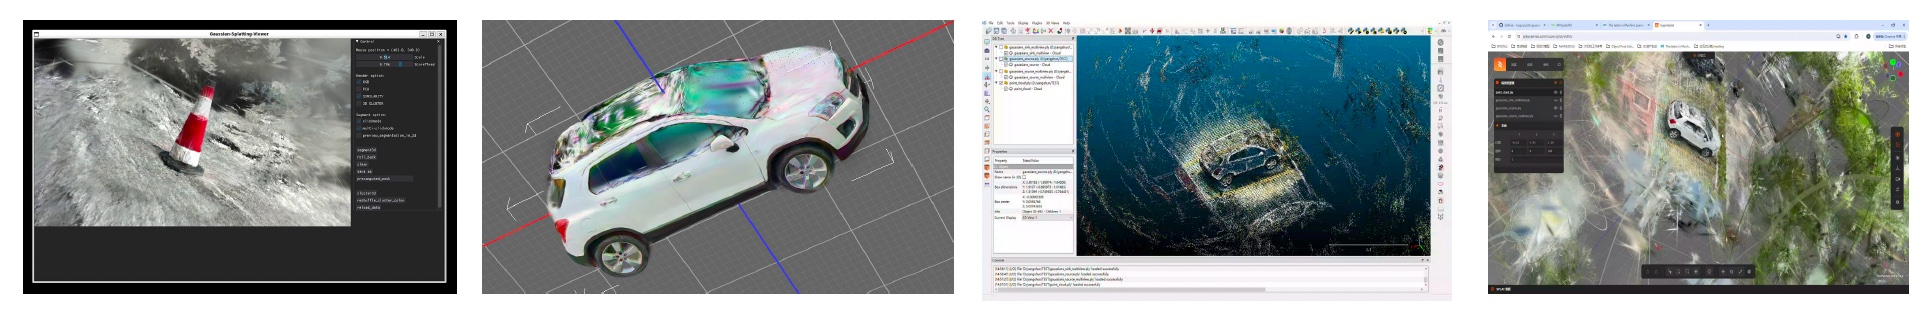
\includegraphics[width=0.95\textwidth]{imgs/gen_3d_object_to_edit.jpeg}
  \caption{3D场景重建与资产提取}
  \label{fig:gen-3d-object}
\end{figure}

\subsection{场景编辑与对象插入}

图~\ref{fig:scene-edit}展示了将重建的3D物体插入到已有场景中的效果。该功能通过在真实场景中添加、移除或修改物体,实现多样化测试场景的构建,是corner case生成的核心技术之一。

场景编辑的关键在于确保插入物体与背景场景的一致性。系统通过组合渲染管线,统一处理背景高斯、物体高斯和天空环境,正确计算遮挡关系和深度排序。通过4DGS的可微分特性,系统优化插入物体的空间变换参数,使其自然融入场景。

从图中可以观察到,插入车辆与背景场景形成了一致的视觉效果,光照匹配合理,边缘过渡自然。系统支持对插入物体进行平移、旋转和缩放等自由变换,为corner case的灵活构建提供了有效工具。场景编辑功能的实现体现了五层解耦架构的优势,系统能够独立管理背景和动态物体,支持灵活的场景组合。生成的编辑场景可有效用于自动驾驶感知和规划算法的训练测试,显著降低了数据采集成本。

\begin{figure}[htbp]
  \centering
  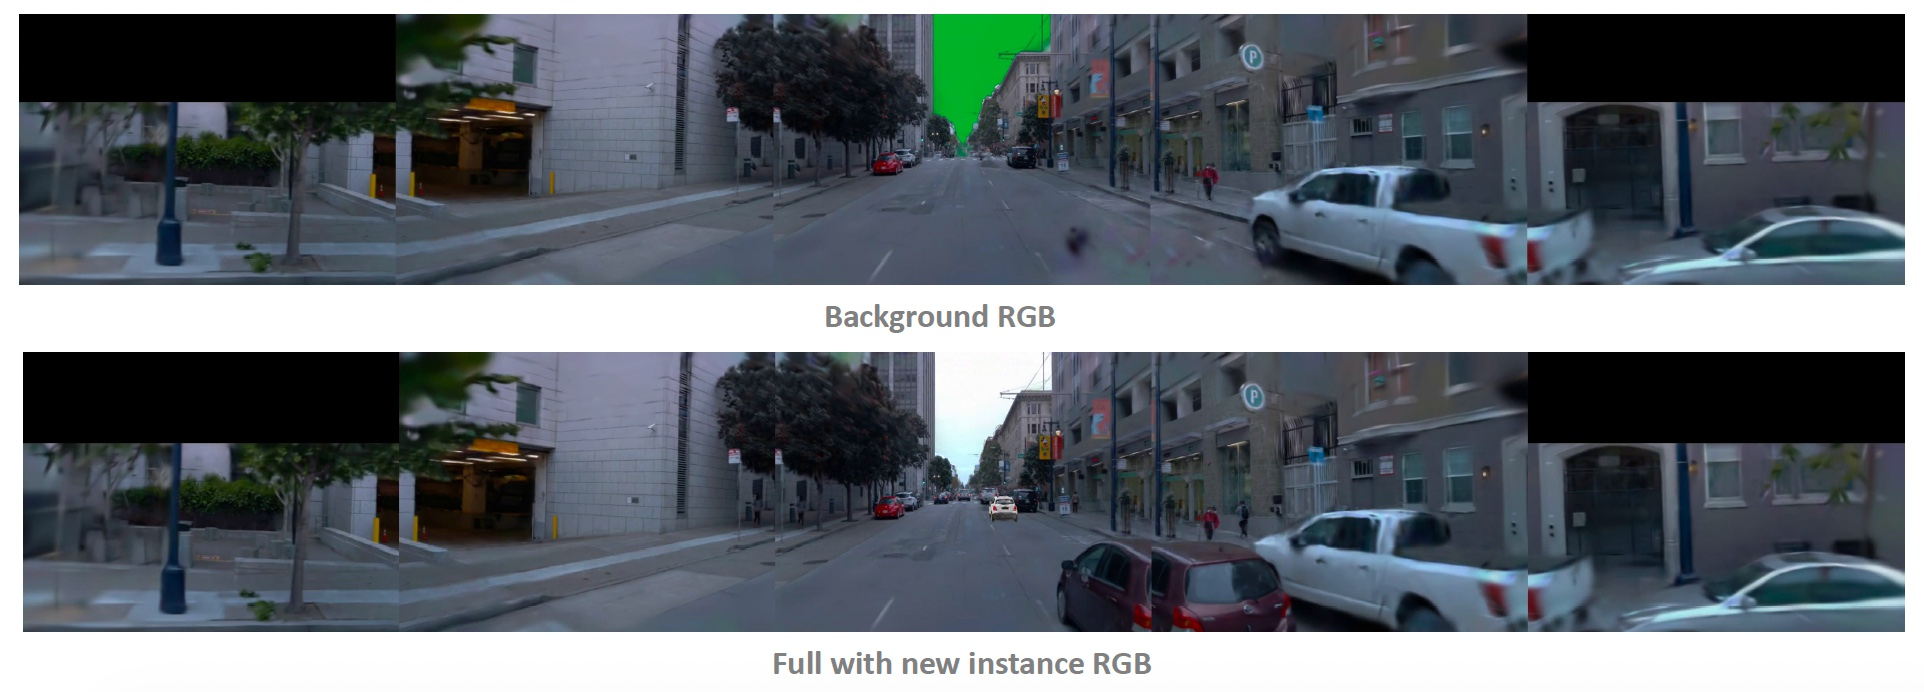
\includegraphics[width=0.95\textwidth]{imgs/3d_scen_edit_with_object.jpeg}
  \caption{场景编辑与对象插入效果}
  \label{fig:scene-edit}
\end{figure}

\subsection{扩散引导训练流程}

图~\ref{fig:training-pipeline}展示了系统从多视角图像到新视角渲染的完整流程,包括数据处理、场景表示构建、扩散引导训练和渲染输出等阶段。

训练流程以多视角图像为输入,经数据预处理生成LiDAR几何条件和相机参数,用于初始化4DGS场景表示。系统构建包含静态背景、动态物体和天空环境的完整场景模型,采用联合优化策略:在训练视点上利用真实图像进行重建损失监督,在新视点上引入扩散模型生成的伪真值进行引导训练。

图中展示的中间结果包括深度图和渲染质量评估等可视化信息。深度图验证了4DGS表示的几何准确性,扩散模型的条件引导为新视点提供了高质量监督信号,克服了传统方法在视点外推时缺乏真值的局限。训练过程采用自适应调度策略,根据模型收敛状态动态调整扩散采样频率和引导强度,确保训练稳定性。

最终渲染结果表明,系统在新视角合成任务上实现了良好的几何一致性和纹理细节。相比仅依靠训练视点监督的方法,引入扩散先验后系统在新视角外推时表现出更强的泛化能力。该流程验证了扩散引导训练策略在提升场景重建质量方面的有效性。

\begin{figure}[htbp]
  \centering
  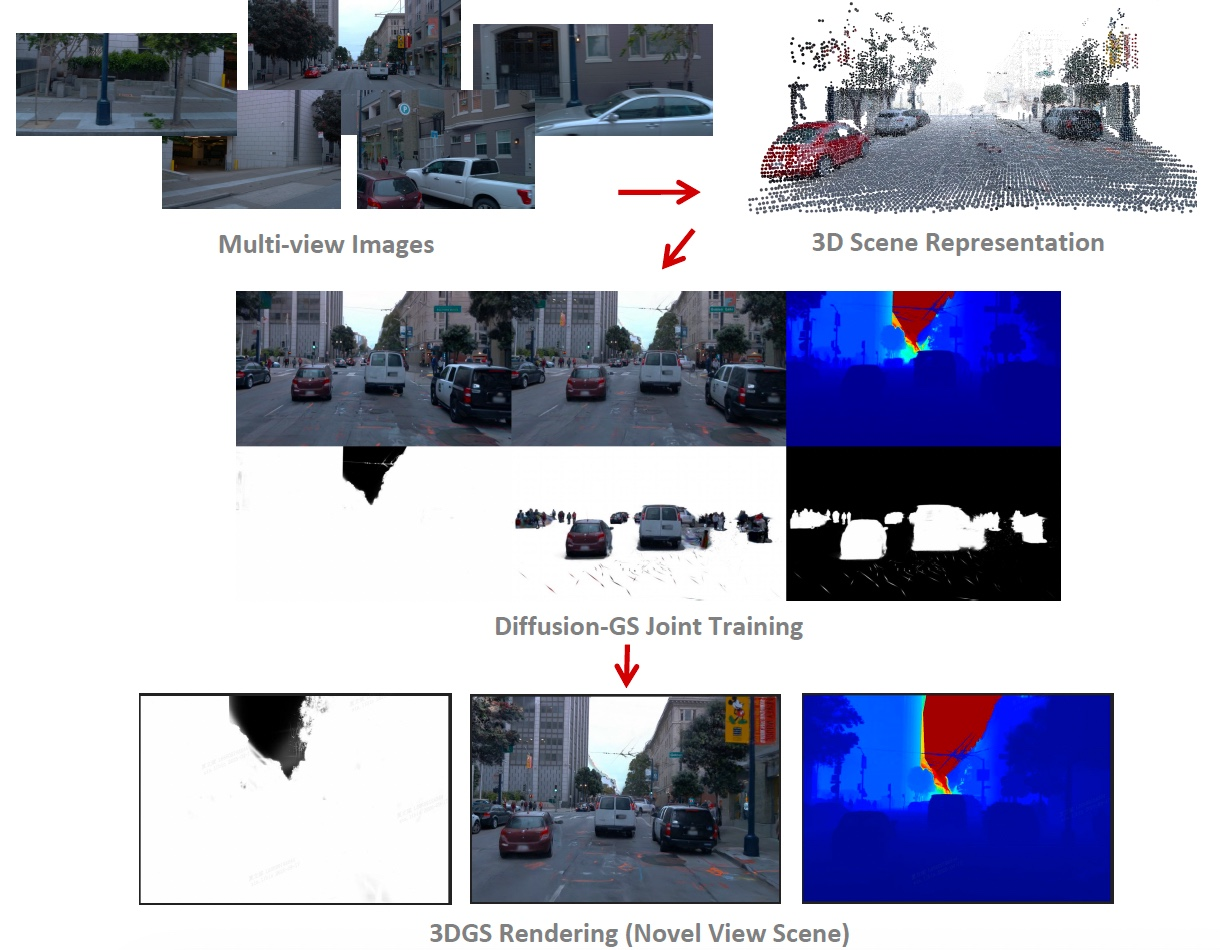
\includegraphics[width=0.95\textwidth]{imgs/from_image_train_to_rendering.jpeg}
  \caption{扩散引导训练与渲染流程}
  \label{fig:training-pipeline}
\end{figure}

\subsection{新视角合成质量对比}

图~\ref{fig:nvs-comparison}对比了不同方法在新视角合成任务上的效果,包括基线方法StreetGS、中间训练阶段结果以及最终的扩散引导方法。对比实验验证了扩散引导策略的有效性。

从对比结果可以观察到各方法的显著差异。StreetGS基线方法在新视角外推时出现明显的模糊和失真,特别是在远离训练视点的区域,图像质量下降明显,细节丢失严重。这反映了传统4DGS方法在缺乏新视点监督时的固有局限性,即过拟合于训练视点而难以泛化到未见区域。中间训练阶段的结果展示了引入扩散引导后的渐进式改善。

最终的扩散引导方法在多个评估维度上表现优异。在几何一致性方面,生成图像准确保持了场景的空间结构,建筑物轮廓清晰,透视关系正确。在纹理细节方面,图像保留了丰富的高频信息,道路标识清晰,车辆表面材质真实。在时序连贯性方面,连续帧之间过渡平滑,未出现明显闪烁或不连续现象。

定性分析表明,扩散先验的引入是质量提升的关键因素。预训练视频扩散模型包含丰富的场景先验知识,能够推理合理的场景结构和纹理细节。通过训练自由引导机制,系统将生成能力传递给4DGS模型,使其在新视点渲染时不仅依赖几何约束,还能利用先验知识进行外推。自适应采样调度策略确保了引导过程的稳定性,避免了过度依赖扩散监督导致的模型退化。对比结果验证了系统设计的有效性。

\begin{figure}[htbp]
  \centering
  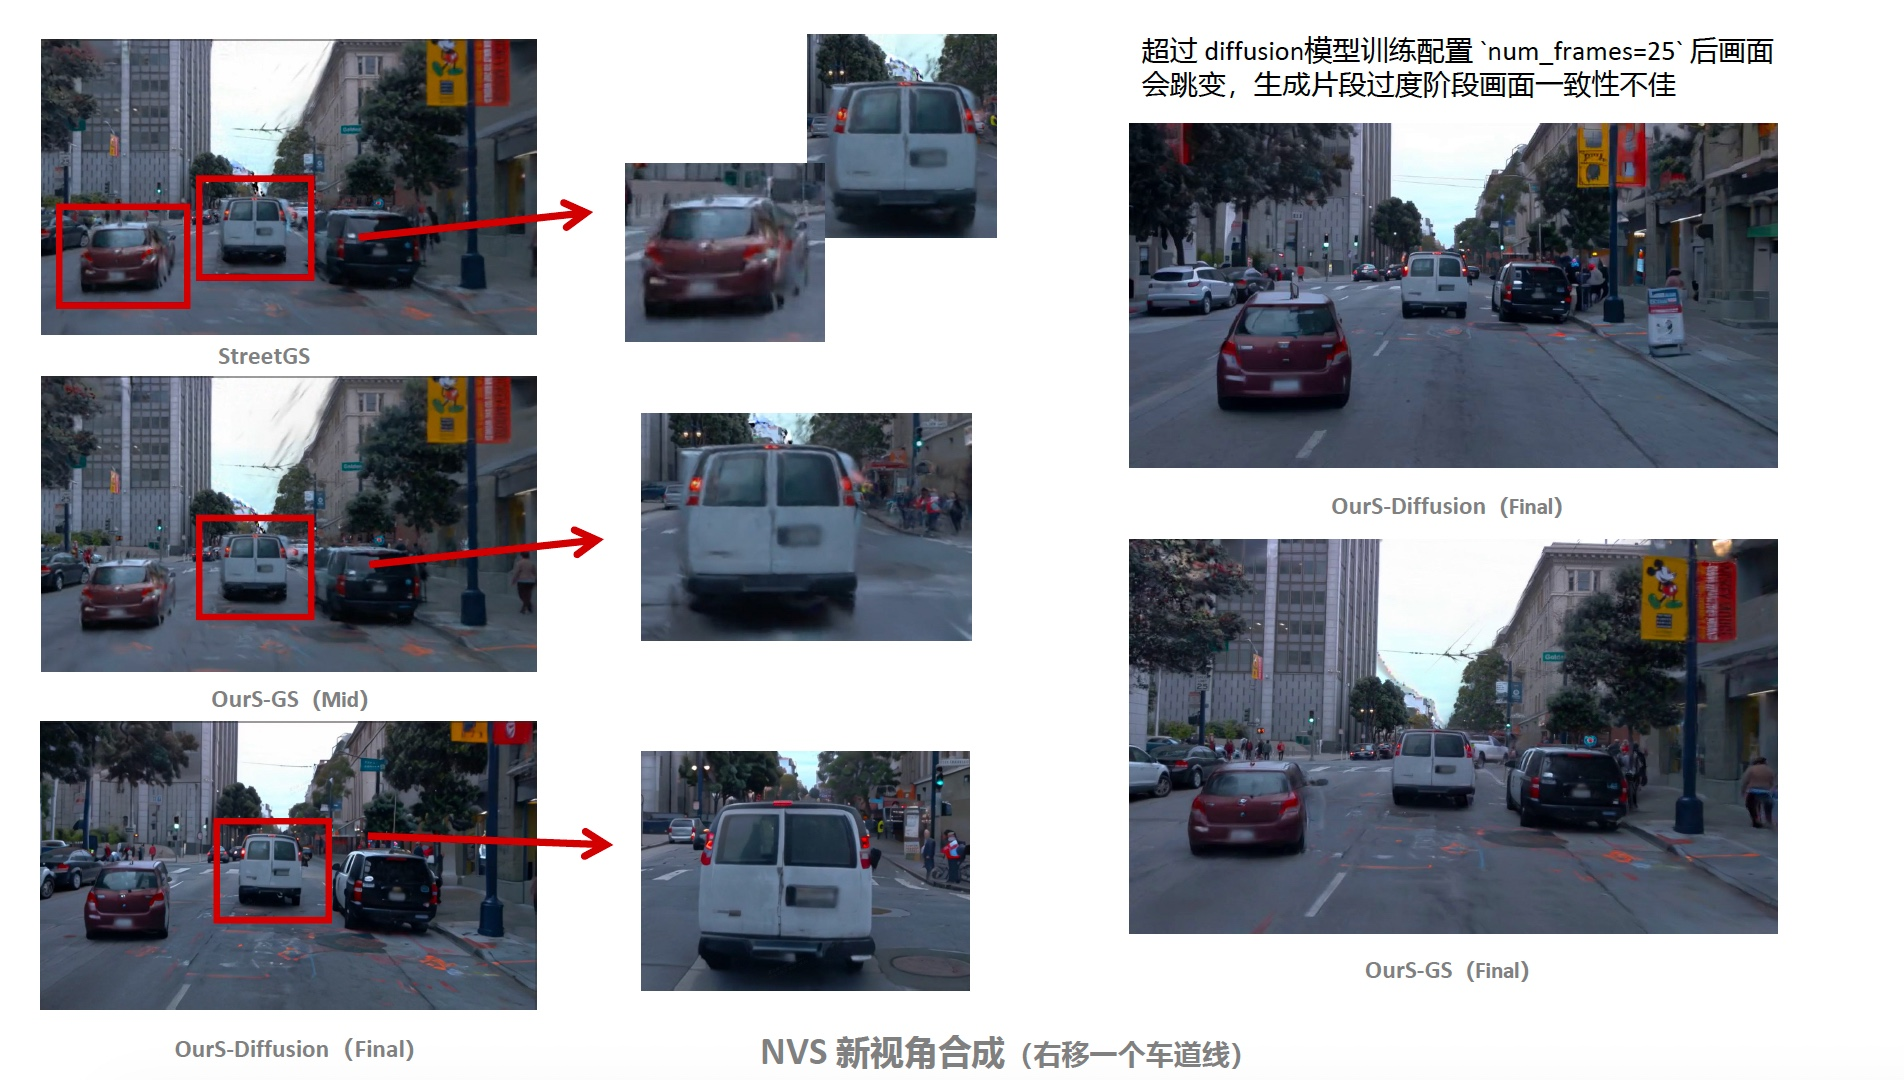
\includegraphics[width=0.95\textwidth]{imgs/nvs_compare_gs_and_diffusion_diffusiongs.jpeg}
  \caption{新视角合成质量对比}
  \label{fig:nvs-comparison}
\end{figure}

\section{本章小结}

本章从系统架构和工程实现的角度,详细阐述了ReGen系统的设计原理和关键技术实现。本文提出的五层解耦架构有效降低了系统复杂度,提高了可维护性和可扩展性。针对4D高斯溅射和视频扩散模型融合的技术挑战,系统设计了多模态渲染管线和GPU加速优化策略,实现了高性能的实时渲染。

在扩散模型集成方面,系统采用了基于Wan2.2-I2V-A14B的Diffusion Transformer架构,通过自适应采样调度和训练自由引导机制实现了高效的扩散监督训练。针对长视频序列处理的内存挑战,系统设计了滑动窗口机制和键值缓存策略,使得系统能够在单个GPU上生成长时长的高分辨率视频序列。

在系统优化方面,系统实现了分层内存管理策略和异步计算流水线,显著提升了训练效率。数值稳定性和收敛性保证机制确保了训练过程的鲁棒性。针对4DGS的动态几何表示需求,本文提出了多准则密化决策算法,综合考虑梯度统计、几何特征和时间一致性来指导高斯基元的动态调整。

在分布式训练方面,系统设计了融合FSDP和Ulysses序列并行的分布式训练架构,通过参数分片、梯度压缩和动态负载均衡策略,支持在多GPU集群上进行大规模模型的高效训练。针对不同的部署需求,系统实现了灵活的多模式推理引擎,支持各种硬件配置和应用场景。

数据处理系统实现了完整的处理管线,包括天空掩码生成、彩色点云融合和LiDAR条件图像生成。质量监控系统通过多维度指标的综合评估,确保了训练过程的稳定性和可靠性。这些系统级的工程创新为高保真4D场景重建的实际应用提供了坚实的技术基础。
